\subsubsection{Hráč JIM}
	\label{jim}
Aktuálnou predlohou hráča, vyvíjanou aj na predmete Tímový projekt, z ktorej bude vychádzať táto práca, je verzia agenta s názvom JIM. Jeho autormi sú 3 absolventi FIIT v roku 2011 - Juraj Drahoš, Ivan Hujsi, Maroš Urbanec. Zo začiatočných písmen ich mien je vytvorený aj názov JIM.

Jadro robota je napísané v objektovo-orientovanom jazyku Java. Jadro tvorí aj najväčšiu časť robota. Pre rozhodovanie a používané schopnosti sú použité Ruby skripty. Pretože jazyk Ruby je interpretovaný jazyk, hráč dokáže načítať súbory pohybov za behu. Ďalšou výhodou Ruby je možnosť meniť parametre pohybu alebo správania bez nutnosti prekompilovať zdrojový kód.

Architektúra agenta je založená na modeli Believe Desire Itention (BDI). Ide o decentralizovanú architektúru, často využívanú v multiagentových prostrediach. Agent  si  na  základe  získaných  vnemov  utvorí  predstavu  o  okolitom   svete  a  na  základe existujúcej  situácie  a  cieľov  si  vytvorí  plán.  Pri  rozhodovaní  sa  teda  riadi  aktuálnym stavom  sveta  a stanovenými  cieľmi.  Úlohou  plánovača je  vytvoriť  plán  zodpovedajúci  obom kritériám.

Architektúra robota JIM pozostáva z 5 komponentov:

\begin{itemize}
	\item \textit{Model komunikácie} - úlohou je komunikovať so serverom a zabezpečovať analýzu správ
	\item \textit{Model parsovania} - parsuje prijaté správy zo servera
	\item \textit{Model sveta} - predstavuje v architektúre BDI časť Believe. V súčasnom stave je rozdelený na 3 časti. Jednotlivé časti sa aktualizujú samostatne na základe správ prijatých zo servera.
		\begin{itemize}
			\item \textit{Agent model} - obsahuje informácie o pozícii hráča, jeho rotácií, rýchlosti a natočení kĺbov.
			\item \textit{World model} - v ňom sa spracúvajú informácie o lopte - jej rýchlosti a pozícii na ihrisku. Ďalšími informáciami sú pozície, rýchlosti ostatných hráčov.
			\item \textit{Environment model} - informácie o hre.
		\end{itemize}
	\item \textit{Plánovací modul} - v architektúre BDI predstavuje časť Desire a Intention. Skladá sa z dvoch častí. Tými sú plánovací algoritmus a vyššie schopnosti. Plánovací algoritmus je možné jednoducho meniť, vďaka spôsobu, akým je architektúra navrhnutá.
	\item \textit{Modul pohybov} - vykonáva požadované pohyb, ktoré dostáva ako príkazy z vyšších schopností a na základe modelu sveta.
\end{itemize}

Tieto komponenty sú navzájom prepojené. Schému architektúry hráča a prepojenie modulov zobrazuje obrázok \ref{pic_jim_architecture}.

\begin{figure}[H]
	\center
	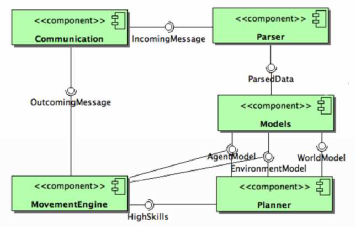
\includegraphics[scale=1]{./data/jim_architecture}
	\caption{Architektúra hráča JIM \cite{durcak}}
	\label{pic_jim_architecture}
\end{figure}